\documentclass{article}
\usepackage[utf8]{inputenc}
\usepackage{pdflscape}
\usepackage{enumerate}

\title{Universidad Nacional Aut\'onoma de M\'exico\\
Facultad de Ciencias\\
Lenguajes de Programación}

\author{Fernando Bernal Mart\'inez }
\date{August 2018}

\usepackage{natbib}
\usepackage{graphicx}




\newenvironment{changemargin}[2]{%
\begin{list}{}{%
\setlength{\topsep}{0pt}%
\setlength{\leftmargin}{#1}%
\setlength{\rightmargin}{#2}%
\setlength{\listparindent}{\parindent}%
\setlength{\itemindent}{\parindent}%
\setlength{\parsep}{\parskip}%
}%
\item[]}{\end{list}} 

\begin{document}

\maketitle

\section{Joseph-Marie Jacquard}

    \subsection{Historia}
    Joseph-Marie Jacquard, (nacido el 7 de julio de 1752,
    Lyon, Francia, murió el 7 de agosto de 1834, Oullins).
    
    Inventor francés del telar Jacquard, como su padre, se convirtió en tejedor de seda y heredó el negocio. Tuvo siempre un gran interés por mejorar los procesos textiles sobre los que trabajaba, observando que los dibujos que se realizaban eran fruto de procesos repetitivos y bastante similares. Sin embargo, con 40 años de edad solamente ya había conseguido fracasar en varios y costosos proyectos que le llevaron  a  la  bancarrota.
    Durante un tiempo se dedicó a otros asuntos, sin embargo, con la
    revolución francesa desarrollándose, apoyó al Antiguo
    Régimen y luchó contra los revolucionarios. Una vez
    finalizada, volvería a Lyon y retomaría su pasión por
    mejorar el trabajo de la seda.[1]\\
    
    Cuando Francia buscaba la forma de hacer frente a la fuerte competencia del sector textil Inglés contrato a Jacques de Vaucanson, quien diseñó en 1745 el primer telar completamente automatizado de la historia. Su prototipo funcionaba con movimientos repetitivos guiados con tarjetas perforadas, pero cuando muri\'o Vaucanson el proyecto quedo abandonado hasta que Jacquard lo descubrió, restauró y perfeccionó en gran medida.
    
    \subsection{Pricipales contribuciones e impacto a las ciencias de la computación}
    Contribuci\'on: Un telar con tarjetas perforadas.\\\\
    La máquina permitía fabricar telas con hilos de distintos colores y complicados dibujos mediante el uso de tarjetas perforadas, y podía ser manejada por un solo operario. Gracias a las innovaciones de Jacquard, los hilos de urdimbre se movían de forma independiente para conseguir el dibujo deseado. También automatizó las 'arcadas' para poder tejer piezas de dibujo complicado.\\
    
    Este dispositivo se gobierna mediante un paquete de tarjetas de cartón perforadas que se cambian accionando un pedal, y que activan un complejo mecanismo de cuerdas y plantas que elevan de forma alternativa un número diferente de hilos de urdimbre para la colocación de los hilos de la trama. Hasta ese momento el mecanismo se tenía que regular a mano cada vez que se cambiaba el dibujo del tejido. El nuevo modelo desplazó a todos los telares antiguos.\\
    
    \textbf{Su idea de las tarjetas perforadas fue adoptada por Charles Babbage para su máquina analítica, y por Herman Hollerith en las tabuladoras, origen de las computadoras digitales modernas.
    }
   \subsection{Contribuciones directas o indirectas al área de los lenguajes de programación.}
      
    Las consecuencias de algo tan simple como un agujero abierto o cerrado continúan en el día de hoy. Las tarjetas perforadas fueron ocupadas para las primeras calculadoras y se convertirían en precursoras del sistema binario sobre el cuál se basaron todos los avances realizados en el mundo de los computadores.\\
    
    Las tarjetas perforadas fue primera forma de programar, ya que desde un inicio, las restricciones de hardware definían el lenguaje. \\
    
    \subsection{Ejemplos}
    En los 60' FORTRAN (FORmula TRANslation system, o Sistema de Traducción de Fórmulas) al escribir un programa se debia perforar una tarjeta por cada línea de código del programa. [4]
   
\section{Digr\'afica: Lenguajes de programaci\'on}
\begin{changemargin}{0cm}{-20cm}
    \begin{landscape}
    
    \begin{figure}

    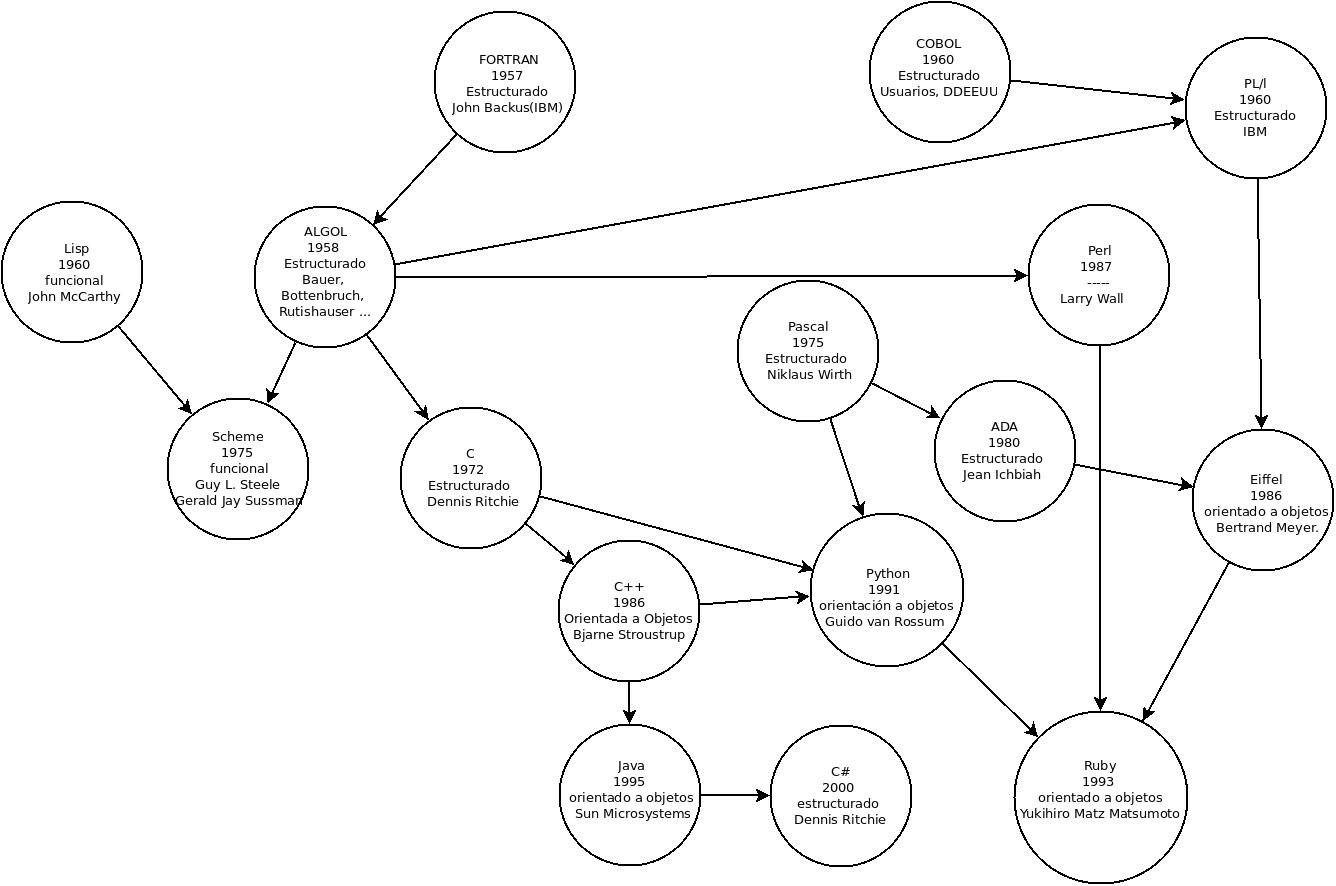
\includegraphics[scale=.48]{tarea1/Diagrama1tarea1-201912.png}
    \caption{Digr\'afica: Lenguajes de Programaci\'on}
    \label{fig:universe}
    \end{figure}
\end{landscape} 
\end{changemargin} 

\section{Ejercicio de investigaci\'on}
\begin{itemize}
    
    \item ¿Por qu\'e se dice que un lenguaje es multiparadigma?\\
    \\Por que es el que soporta más de un paradigma de programación. Según lo describe Bjarne Stroustrup, permiten crear “programas usando más de un estilo de programación”.[5]

El objetivo en el diseño de estos lenguajes es permitir a los programadores utilizar el mejor paradigma para cada trabajo, admitiendo que ninguno resuelve todos los problemas de la forma más fácil y eficiente posible. 
    \item ¿Existe el paradigma multiparadigma? Justificar tu respuesta\\
       \\ No, ya que principalmente un paradigma  de programación representa un enfoque particular o filosofía para diseñar soluciones, adem\'as los paradigmas difieren unos de otros, en los conceptos y la forma de abstraer los elementos involucrados en un problema, así como en los pasos que integran su solución del problema.[5]
        
        Decir multiparadigma, significa que tiene un enfoque particular y multiparadigma no es asi, ya que mutiparadiga encapsula los paradigmas (declarativo, orientado  objetos, etc.)  a los cuales un lenguaje puede ser utilizao para manejar un problema.
\end{itemize}



\bibliographystyle{plain}
\begin{thebibliography}{X}
\textit{[1]Encyclopedia Britanica}\\
\textit{By: The Editors of Encyclopaedia Britannica}\\
\textit{https://www.britannica.com/biography/Joseph-Marie-Jacquard}\\
\textit{Consultado el Día: 14 de agosto de 2018}\\
\\
\textit{[2]Jacquard, el tejedor informático}\\
\textit{By: Nuria Martínez Medina}\\
\textit{http://www.rtve.es/noticias/20110923/jacquard-tejedor-informatico/463573.shtml}\\
\textit{Consultado el Día: 14 de agosto de 2018}\\
\\
\textit{[3]Arquitectura de las computadoras}\\
\textit{None}\\
\textit{https://arquitecturacomputadoreshoy.wordpress.com/tag/lenguajes-de-programacion/}\\
\textit{Consultado el Día: 14 de agosto de 2018}\\
\\
\textit{[4]La época de las tarjetas perforadas - BLOGS, La Prensa Grafica}\\
\textit{None}\\
\textit{ http://blogs.laprensagrafica.com/litoibarra/?p=2808}\\
\textit{Consultado el Día: 14 de agosto de 2018}\\
\\
\textit{[5]Wikipedia enciclopedia libre}\\
\textit{None}\\
\textit{https://es.wikipedia.org/wiki/Lenguaje_de_programaci\%C3\%B3nmultiparadigma}\\
\textit{Consultado el Día: 14 de agosto de 2018}\\
\\
\textit{[6]Lenguajes y Paradigmas de Programación}\\
\textit{None}\\
\textit{http://www.dccia.ua.es/dccia/inf/asignaturas/LPP/2008-2009/tema-01.html}\\
\textit{Consultado el Día: 14 de agosto de 2018}\\
\\
\textit{[7]Computer Languages History}\\
\textit{None}\\
\textit{https://www.levenez.com/lang/}\\
\textit{Consultado el Día: 14 de agosto de 2018}\\

\end{thebibliography}
\end{document}

